\documentclass{article}
\usepackage{amssymb, amssymb, amsthm}
\usepackage{natbib}
\usepackage{graphicx}


\author{Elnur Gasanov : 163411}
\title{Homework 2: Bayesian Regression}

\newcommand{\mm}{\bold{m}}
\newcommand{\mS}{\bold{S}}
\newcommand{\mPhi}{\bold{\Phi}}
\newcommand{\mw}{\bold{w}}
\newcommand{\mt}{\bold{t}}
\newcommand{\mI}{\bold{I}}

\parindent=0.0mm

\begin{document}

\maketitle

\section{Derivation of $\mm_N$ and $\mS_N$}

Let us recall that $p (\mt |\mw)$ and $p(\mw)$ have the following forms:

$$
p (\mt |\mw) = \left(\frac{\beta}{2 \pi} \right)^\frac{N}{2} \exp \left\{- \frac\beta2 ||\mt - \mPhi\mw||^2_2 \right\}, 
$$
$$
p(\mw) = \frac{1}{(2\pi)^{\frac{M}{2}} \sqrt{\det \mS_0}} \exp \left\{ -\frac12 (\mw - \mm_0) \mS_0^{-1} (\mw - \mm_0) \right\}.
$$

We will use the fact that "due to the choice of a conjugate Gaussian prior distribution, the posterior will also be Gaussian" \cite{bishop}, \textit{i.e.} $p(\mw |\mt) = \mathcal{N}(\mm_N, \mS_N)$. Due to Bayes rule, 

$$
p(\mw |\mt)~\sim~p(\mt|\mw) p(\mw) \sim \ \exp \left\{- \frac\beta2 ||\mt - \mPhi\mw||^2_2 -\frac12 (\mw - \mm_0) \mS_0^{-1} (\mw - \mm_0) \right\} = .
$$
$$
\exp \left\{ -\frac12 \left(\beta ||\mt||^2_2 - 2 \beta \mt^\intercal \mPhi \mw + \beta \mw^\intercal \mPhi^\intercal \mPhi \mw + \mm_0^\intercal \mS_0^{-1} \mm_0 - 2 \mm_0^\intercal \mS_0^{-1} \mw + \mw^\intercal \mS_0^{-1} \mw \right) \right\} = 
$$
$$
\exp \left\{ -\frac12 \left(  \mw^\intercal (\mS_0^{-1} + \beta \mPhi^\intercal \mPhi) \mw  - 2 (\mm_0^\intercal \mS_0^{-1} + \beta \mt^\intercal \mPhi ) \mw+ const \right) \right\}.
$$

Since $p(\mw |\mt) = \mathcal{N}(\mm_N, \mS_N) \sim \exp \left\{ -\frac{1}{2} \left( \mw^\intercal \mS_N^{-1} \mw - 2 \mm_N^\intercal \mS_N^{-1} \mw \right) \right\}$, we enforce corresponding quadratic form and linear function of $\mw$ to be equal. Therefore,

$$
\mS_N^{-1} = \mS_0^{-1} + \beta \mPhi^\intercal \mPhi.
$$
$$
\mm_N^\intercal \mS_N^{-1} = \mm_0^\intercal \mS_0^{-1} + \beta \mt^\intercal \mPhi 
$$

Second formula after transposition leads to 

$$
\mm_N = \mS_N (\mS_0^{-1} \mm_0 + \beta \mPhi^\intercal \mt).
$$

\section{Sequential Bayesian learning}

Chosen function is $h(x) = 0.2 + 0.5 x $. A gaussian noise with standard deviation 0.1 was added to function values. $p(\mw) = \mathcal{N}(\bold{0}, 0.1 \cdot \mI)$. Obtained graphs are illustrated on figures~\ref{from_scr} and \ref{seq}. The last row of each figure represent learned regression after considering 60 points. Figure \ref{seq}, which represents regressions learned in sequential fashion (mean and covariance matrices of posterior distribution are derived from ones on the previous step and new sampled point), shows computational instability of such approach. 

\begin{figure*}
	\centering
	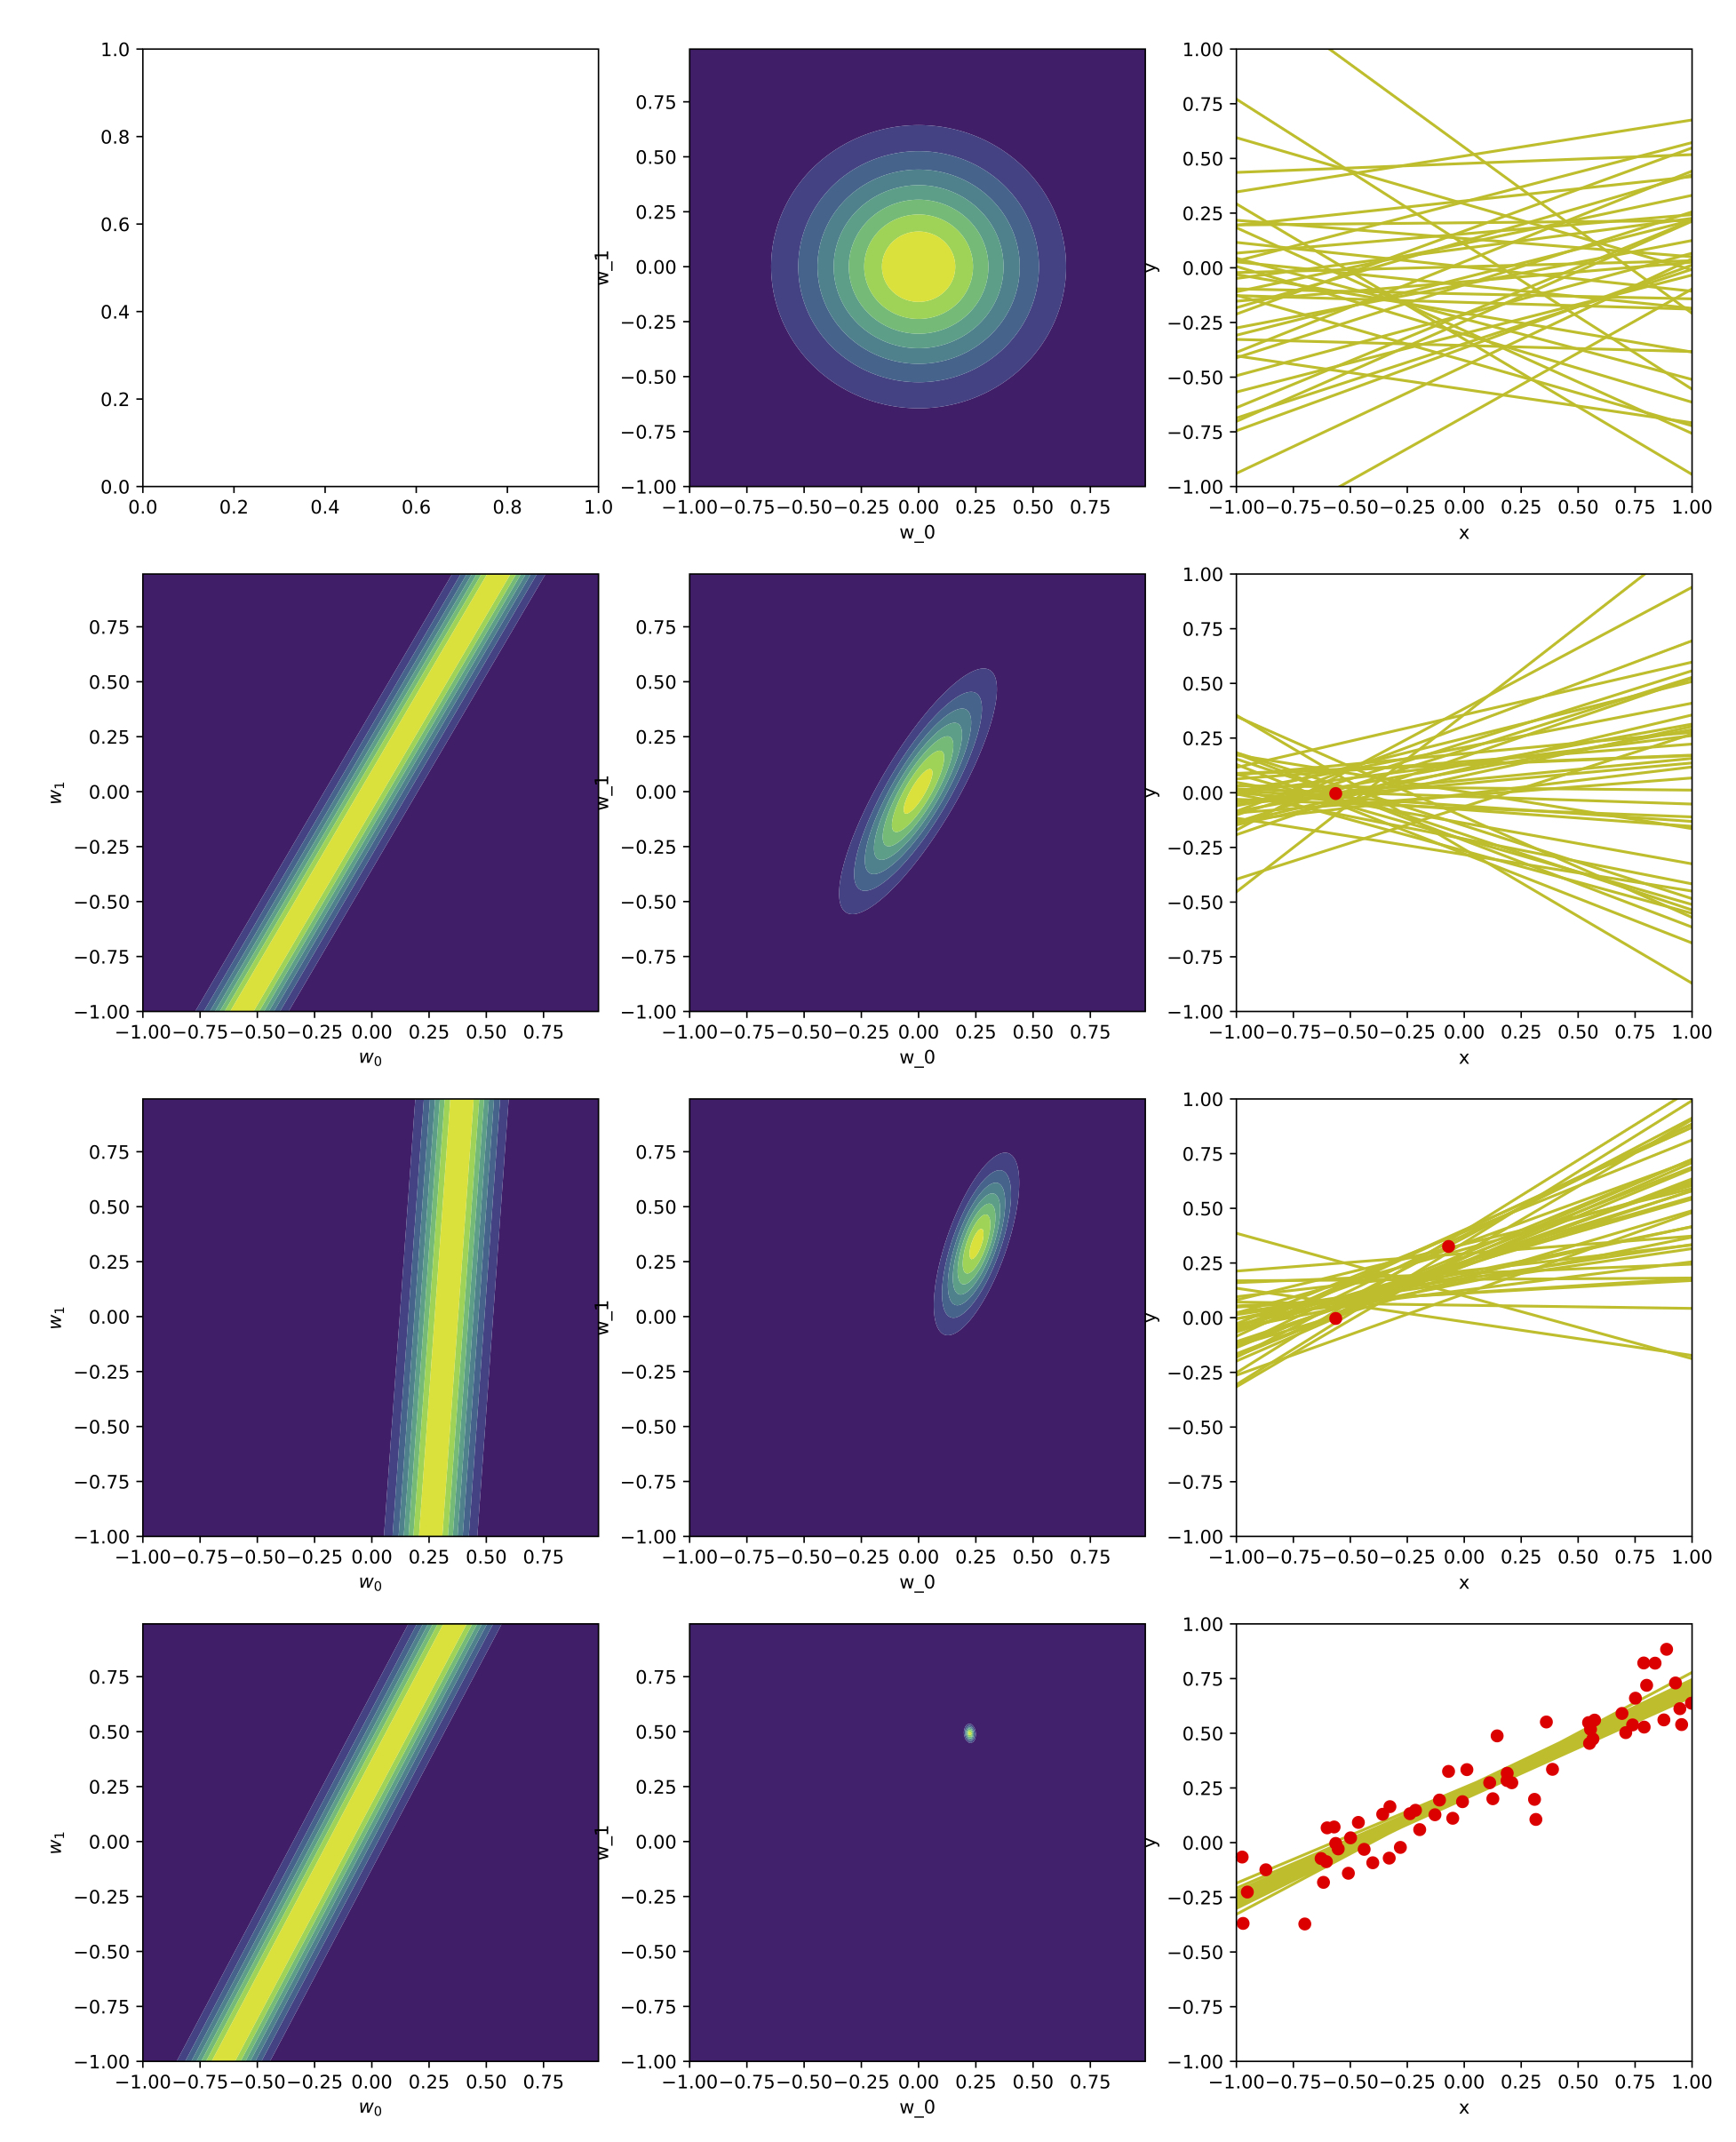
\includegraphics[width=\textwidth]{bayesL.jpg}
	\caption{Illustration of sequential Bayesian learning (matrices (mean, covariance) are recomputed from scratch}
	\label{from_scr}
\end{figure*}
\begin{figure*}
	\centering
	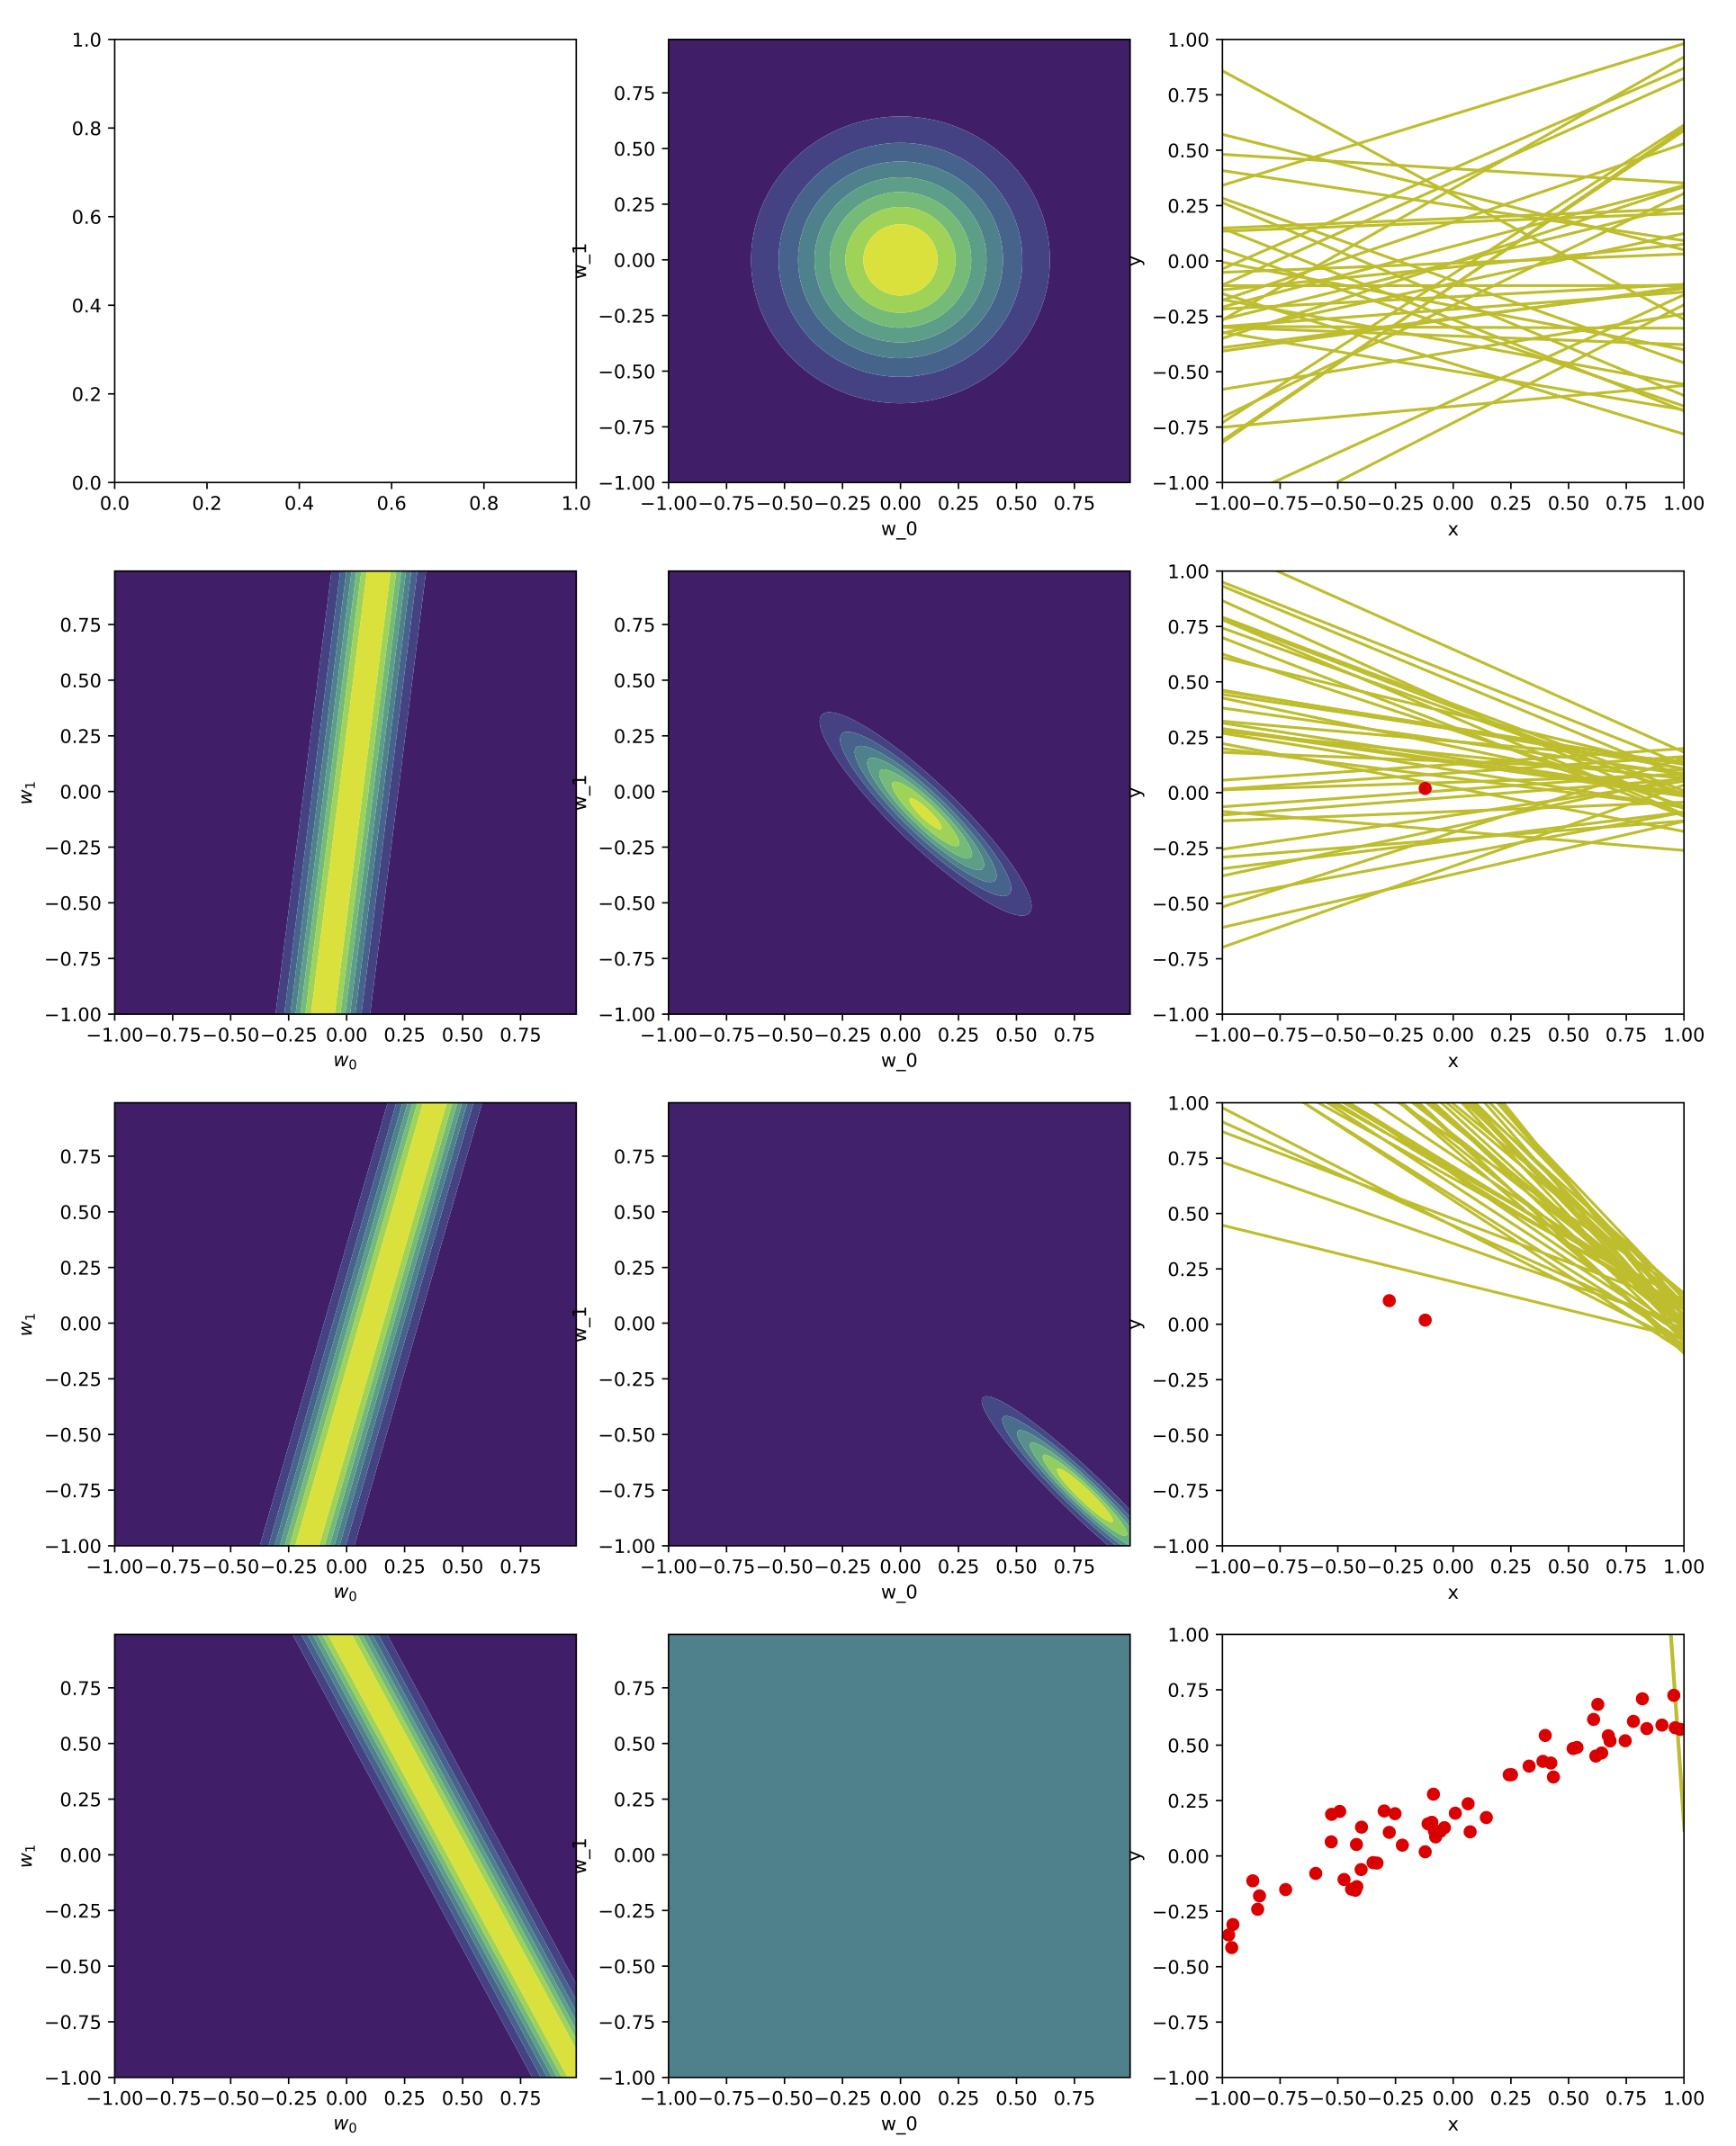
\includegraphics[width=\textwidth]{seq_bayesl.jpg}
	\caption{Illustration of sequential Bayesian learning (matrices are computed sequentially}
	\label{seq}
\end{figure*}




\bibliographystyle{plain}
\bibliography{references}

\end{document}